\chapter{Energia nei decadimenti}

Andiamo a considerare un decadimento in cui una particella $X$ decade in $N$ corpi $Y_i$ del tipo 
%
\begin{equation}
    X \to Y_1 + Y_2 + \cdots + Y_N
\end{equation}
Per descrivere ogni $Y_i$ sarà necessario saperne il quadrimpulso, il quale ha $4$ variabili, questo comporta che per descrivere il sistema formato da $N$ particelle saranno necessarie $4N$ variabili, tuttavia le relazioni $(p^{\mu}_i)^2 = m_i^2$ e $p^{\mu}_X = \sum_i^N p^{\mu}_i$ mi permettono di togliere rispettivamente $N$ e $4$ variabili.\\
Allora i gradi di libertà del sistema risultano essere
%
\begin{equation}
    n_{\text{dof}} = 3N - 4
\end{equation}
Il conteggio dei gradi di libertà si interpreta facilmente. 

Nel caso $N = 2$ si ha $n_{\text{dof}} = 2$, e i due gradi di libertà residui sono i due angoli che individuano la direzione di emissione nel sistema del centro di massa: non resta alcuna libertà sulle energie, che sono quindi \emph{fissate} dalle sole masse in gioco. Lo spettro osservato è in questo caso a righe. 

Per $N = 3$ si ha invece $n_{\text{dof}} = 5$: tre di questi descrivono ancora l'orientazione complessiva dello stato finale, ma ne restano due liberi, che possono essere scelti come le energie di due delle tre particelle. L'energia di ciascun prodotto non è quindi più determinata e può assumere con continuità tutti i valori di un intervallo, compatibilmente con la conservazione dell'energia totale. Lo spettro risulta allora \emph{continuo}, con un valore massimo fissato dall'energia disponibile. 

\section{Decadimento a 2 corpi}

Consideriamo un decadimento a $2$ corpi 
%
\begin{equation}
    X \to Y_1 + Y_2
\end{equation}
Per studiare questo sistema conviene passare al centro di massa in cui i quadrimpulsi sono 
%
\begin{equation*}
    p_X^{\mu} = (m_X, \mathbf{0}) \quad, \quad p_1^{\mu} = (E_1, \mathbf{p}) \quad, \quad p_2^{\mu} = (E_2, - \mathbf{p})  
\end{equation*}

Sfruttando la conservazione del quadrimpulso totale si ottiene facilmente che 

\begin{tcolorbox}[colback=yellow!10!white, colframe=orange!70!black, boxrule=0.8pt]
\begin{equation}
    E_1 = \frac{m_X^2 + m_1^2 - m_2^2}{2 m_X} \quad , \quad E_2 = \frac{m_X^2 + m_2^2 - m_1^2}{2m_X}
\end{equation}
\end{tcolorbox}
%
Negli esperimenti, però, non si misura tutta l'energia della particella, cosa che implicherebbe la sua annichilazione, ma si misura la sua energia cinetica $T_i = E_i - m_i$, che dalle relazioni precedenti risulta essere
%
\begin{equation}
    T_i = \frac{(m_X - m_i)^2 - m_j^2}{2m_X}
\end{equation}

Andiamo adesso ad analizzare in dettaglio due decadimenti a $2$ corpi molto importanti: decadimento $\alpha$ e decadimento $\gamma$.

\subsection{Decadimento $\alpha$}

Un decadimento $\alpha$ è un decadimento a $2$ corpi del tipo 
%
\begin{equation*}
    {}^{A}_{Z}\mathrm{X} \longrightarrow {}^{A-4}_{Z-2}\mathrm{Y} + \alpha \qquad \alpha = {}^{4}_{2}\mathrm{He}
\end{equation*}
Definiamo l'energia di decadimento\mkeyword{energia di decadimento} come la differenza tra la massa del nucleo padre e quelle dei prodotti
%
\begin{equation}
    Q = m_X - m_Y - m_{\alpha}
\end{equation}
Questa quantità è direttamente accessibile all'esperimento. Dalla conservazione dell'energia, infatti, 
%
\begin{equation}
    m_X = T_Y + m_Y + T_{\alpha} + m_{\alpha} \qquad \Longrightarrow \qquad Q = T_Y + T_{\alpha}
\end{equation}
cioè $Q$ coincide con l'energia cinetica totale dei prodotti, misurabile in laboratorio.\\

Vediamo adesso che per studiare questo tipo di decadimento \emph{non sempre} è necessario ricorrere alla meccanica relativistica. Consideriamo come esempio il decadimento 
%
\begin{equation*}
    {}^{238}_{92}\mathrm{U} \longrightarrow {}^{234}_{90}\mathrm{Th} + \alpha
\end{equation*}
per il quale si ha $Q = 5$ MeV. Possiamo stimare le masse in gioco come 
%
\begin{equation}
    m_i = A_i \, u \qquad u = 1 \ \mathrm{GeV}
\end{equation}
dove $u$ è l'unità di massa atomica e $A_i$ il numero di massa. Nel nostro caso si ottiene 
%
\begin{equation}
    m_{X,Y} \approx 200 \ \mathrm{GeV} \ , \qquad m_{\alpha} = 4 \ \mathrm{GeV}
\end{equation}
L'energia di massa è quindi di diversi ordini di grandezza maggiore dell'energia cinetica in gioco: le particelle si muovono a velocità non relativistiche e possiamo trattare il problema in meccanica classica. 

Bastano allora le relazioni 
%
\begin{equation}
\begin{cases}
    Q = T_{\alpha} + T_Y \\[4pt]
    T_{\alpha} = \dfrac{p^2}{2m_{\alpha}} \qquad \Longrightarrow \qquad p^2 = 2 m_{\alpha} T_{\alpha} \\[8pt]
    T_Y = \dfrac{p^2}{2m_Y} = \dfrac{m_{\alpha}}{m_Y} T_{\alpha}
\end{cases}
\end{equation}
dove si è usato il fatto che, essendo il nucleo padre inizialmente in quiete, i due prodotti hanno impulsi opposti e di uguale modulo $p$. Sostituendo si ricava
%
\begin{equation}
    Q = T_{\alpha} \left( 1 + \frac{m_{\alpha}}{m_Y} \right)
\end{equation}

Invertendo quest'ultima relazione si ottiene l'energia cinetica della particella $\alpha$ in funzione di $Q$
%
\begin{tcolorbox}[colback=yellow!10!white, colframe=orange!70!black, boxrule=0.8pt]
\begin{equation}
    T_{\alpha} = \frac{m_Y}{m_{\alpha} + m_Y} \, Q = \frac{A-4}{A} \, Q
\end{equation}
\end{tcolorbox}
e, per differenza, quella del nucleo di rinculo
%
\begin{tcolorbox}[colback=yellow!10!white, colframe=orange!70!black, boxrule=0.8pt]
\begin{equation}
    T_Y = \frac{m_{\alpha}}{m_{\alpha} + m_Y} \, Q = \frac{4}{A} \, Q
\end{equation}
\end{tcolorbox}
dove si sono usate le stime $m_{\alpha} = 4u$ e $m_Y = (A-4)u$. 

Dato che per gli emettitori $\alpha$ si ha $A \gg 4$, questo significa che è la particella $\alpha$ a prendersi praticamente tutta l'energia cinetica disponibile, mentre al nucleo figlio ne resta solo una frazione dell'ordine di $4/A$.

\subsection{Decadimento $\gamma$}

Un decadimento $\gamma$ è un decadimento a $2$ corpi in cui un nucleo in uno stato eccitato si diseccita emettendo un fotone
%
\begin{equation*}
    {}^{A}_{Z}\mathrm{X}^* \longrightarrow {}^{A}_{Z}\mathrm{X} + \gamma
\end{equation*}
A differenza dei casi precedenti il nuclide non cambia: variano soltanto l'energia e lo stato di eccitazione del nucleo. Un esempio è
%
\begin{equation*}
    {}^{152}_{62}\mathrm{Sm}^* \longrightarrow {}^{152}_{62}\mathrm{Sm} + \gamma
\end{equation*}

Indichiamo con $M$ la massa del nucleo eccitato e con $\Delta$ l'energia di eccitazione, cosicché il nucleo nello stato finale ha massa $M - \Delta$. Trattandosi di un decadimento a due corpi possiamo usare direttamente la relazione ricavata in precedenza
%
\begin{equation*}
    E_1 = \frac{M^2 + m_1^2 - m_2^2}{2M}
\end{equation*}
sostituendo $m_1 = 0$ per il fotone e $m_2 = M - \Delta$ per il nucleo figlio. Si ottiene allora
%
\begin{tcolorbox}[colback=yellow!10!white, colframe=orange!70!black, boxrule=0.8pt]
\begin{equation}
    E_{\gamma} = \frac{M^2 - (M-\Delta)^2}{2M} = \Delta - \frac{\Delta^2}{2M}
\end{equation}
\end{tcolorbox}
e, per il nucleo,
%
\begin{equation}
    E_{\mathrm{Sm}} = \frac{M^2 + (M-\Delta)^2}{2M} = M - \Delta + \frac{\Delta^2}{2M}
\end{equation}
Dalla forma di $E_{\mathrm{Sm}}$ si ricava immediatamente la sua energia cinetica, cioè l'energia di rinculo
%
\begin{tcolorbox}[colback=yellow!10!white, colframe=orange!70!black, boxrule=0.8pt]
\begin{equation}
    T_{\mathrm{Sm}} = E_{\mathrm{Sm}} - (M - \Delta) = \frac{\Delta^2}{2M}
\end{equation}
\end{tcolorbox}
Il fotone si porta quindi via quasi tutta l'energia di eccitazione, $E_{\gamma} \simeq \Delta$, mentre al nucleo resta soltanto il termine di rinculo $\Delta^2/2M$, piccolissimo dato che $\Delta \ll M$.

\section{Decadimento a 3 corpi}

Consideriamo un decadimento a $3$ corpi 
%
\begin{equation}
    X \to Y_1 + Y_2 + Y_3
\end{equation}
Come visto all'inizio del capitolo, in questo caso $n_{\text{dof}} = 5$: tre gradi di libertà fissano l'orientazione complessiva dello stato finale, mentre i due rimanenti restano liberi e possono essere scelti come le energie di due delle tre particelle. 

Il motivo per cui l'energia non è più determinata si vede bene ripetendo il conto fatto nel caso a due corpi. Nel sistema di quiete di $X$ si ha
%
\begin{equation*}
    p_X^{\mu} = (m_X, \mathbf{0}) \qquad \Longrightarrow \qquad (p_X^{\mu} - p_1^{\mu})^2 = (p_2^{\mu} + p_3^{\mu})^2
\end{equation*}
Sviluppando il primo membro e chiamando $m_{23}^2 = (p_2^{\mu} + p_3^{\mu})^2$ la massa invariante del sistema formato dalle altre due particelle, si ottiene
%
\begin{tcolorbox}[colback=yellow!10!white, colframe=orange!70!black, boxrule=0.8pt]
\begin{equation}
    E_1 = \frac{m_X^2 + m_1^2 - m_{23}^2}{2 m_X}
\end{equation}
\end{tcolorbox}
La formula è formalmente identica a quella del caso a due corpi, con la differenza fondamentale che al posto della massa $m_2$ compare ora $m_{23}$. Mentre $m_2$ è una costante fissata dalla natura della particella, $m_{23}$ \emph{non è una costante}: dipende da come le particelle $2$ e $3$ si ripartiscono energia e impulso, e quindi cambia da evento a evento. 

I valori che può assumere sono limitati dalla cinematica
%
\begin{equation}
    m_2 + m_3 \leq m_{23} \leq m_X - m_1
\end{equation}
dove il minimo si ha quando le particelle $2$ e $3$ sono in quiete l'una rispetto all'altra e il massimo quando è la particella $1$ a essere emessa con impulso nullo. 

Di conseguenza l'energia della particella $1$ può assumere con continuità tutti i valori dell'intervallo
%
\begin{equation}
    m_1 \leq E_1 \leq \frac{m_X^2 + m_1^2 - (m_2+m_3)^2}{2 m_X}
\end{equation}
Lo spettro è quindi \emph{continuo} e non a righe: la cinematica da sola fissa soltanto gli estremi dell'intervallo, mentre la distribuzione delle energie al suo interno è determinata dalla dinamica del processo. \\

Andiamo ad analizzare in dettaglio il decadimento a tre corpi più importante: decadimento $\beta$. 

\newpage

\subsection{Decadimento $\beta$}

Il decadimento $\beta$ è il tipico decadimento a $3$ corpi
%
\begin{equation*}
    {}^{A}_{Z}\mathrm{X} \longrightarrow {}^{A}_{Z+1}\mathrm{Y} + e^- + \bar{\nu}_e
\end{equation*}
un esempio del quale è il decadimento del trizio
%
\begin{equation*}
    {}^{3}_{1}\mathrm{H} \longrightarrow {}^{3}_{2}\mathrm{He} + e^- + \bar{\nu}_e \qquad Q = 18 \ \mathrm{keV}
\end{equation*}

Dei tre prodotti, il neutrino non può essere misurato facilmente e il rinculo del nucleo è a sua volta difficile da misurare: in pratica l'unica quantità accessibile è l'energia dell'elettrone. Quello che si ottiene da un esperimento è quindi il numero di elettroni emessi in un intervallo di energia, cioè
%
\begin{equation}
    dN = f(E) \, dE \qquad \Longrightarrow \qquad \frac{dN}{dE} = f(E)
\end{equation}
dove $f(E)$ è una densità, e il numero di elettroni emessi in un intervallo finito si ottiene integrando
%
\begin{equation*}
    N = \int_{E_{min}}^{E_{max}} \frac{dN}{dE} \, dE
\end{equation*}
Come visto sopra, la cinematica da sola non basta a determinare la forma di questa distribuzione: fissa soltanto l'intervallo in cui l'energia può variare. Per ricavarne la forma occorre la \emph{regola d'oro di Fermi}\mkeyword{regola d'oro di Fermi}
%
\begin{tcolorbox}[colback=yellow!10!white, colframe=orange!70!black, boxrule=0.8pt]
\begin{equation}
    \Gamma_{i \to f} = \frac{2\pi}{\hbar} \left| \langle f | H | i \rangle \right|^2 \rho(E_f)
\end{equation}
\end{tcolorbox}
che fornisce la probabilità di transizione $i \to f$ per unità di tempo. Il primo fattore è l'elemento di matrice dell'interazione responsabile del decadimento e contiene tutta la \emph{dinamica} del processo, mentre $\rho(E_f) = dn/dE_f$ è la densità degli stati finali, cioè il numero di stati accessibili per unità di energia, e dipende solo dalla \emph{cinematica}. 

L'uso della regola d'oro è giustificato dal fatto che l'interazione responsabile del decadimento è debole rispetto a quella che forma gli stati nucleari: i tempi caratteristici del decadimento $\beta$, dell'ordine del secondo o maggiori, sono enormemente più lunghi del tempo nucleare caratteristico ($\sim 10^{-20}$ s), e l'interazione può quindi essere trattata come una perturbazione.\\

Per ricavare la forma dello spettro assumiamo che l'elemento di matrice non dipenda dagli impulsi dei prodotti. Questa è l'\emph{approssimazione permessa}\mkeyword{approssimazione permessa}: le funzioni d'onda dell'elettrone e del neutrino sono onde piane $e^{i \mathbf{p} \cdot \mathbf{r}/\hbar}$ e, poiché sul volume nucleare si ha $pr \ll \hbar$, possiamo svilupparle tenendo solo il primo termine
%
\begin{equation}
    e^{i \mathbf{p} \cdot \mathbf{r}/\hbar} = 1 + \frac{i \mathbf{p} \cdot \mathbf{r}}{\hbar} + \cdots \simeq 1
\end{equation}
In questa approssimazione l'unica dipendenza dall'energia resta quella dello spazio delle fasi, e tutto il problema si riduce a contare gli stati finali disponibili.\\

Il numero di stati accessibili all'elettrone con impulso compreso tra $p$ e $p+dp$, in un volume di normalizzazione $V$, è
%
\begin{equation}
    dn_e = \frac{4 \pi p^2 \, dp \, V}{h^3}
\end{equation}
dove il fattore $h^3$ è il volume elementare dello spazio delle fasi e rende il risultato un numero puro. Analogamente, per il neutrino di impulso $q$,
%
\begin{equation}
    dn_{\nu} = \frac{4 \pi q^2 \, dq \, V}{h^3}
\end{equation}
Il numero di stati finali che hanno simultaneamente un elettrone e un neutrino con gli impulsi voluti è il prodotto dei due
%
\begin{equation}
    d^2 n = dn_e \, dn_{\nu} = \frac{(4\pi)^2 V^2 p^2 q^2 \, dp \, dq}{h^6} \propto p^2 q^2 \, dp \, dq
\end{equation}
Si noti che fino a questo punto non si è ancora usata la conservazione dell'energia: $p$ e $q$ sono stati trattati come indipendenti. Imponendola, e trascurando l'energia di rinculo del nucleo, si ha
%
\begin{equation}
    Q = T + T_{\nu} \qquad \text{e} \qquad T_{\nu} = q
\end{equation}
dove si è usato $m_{\nu} = 0$\footnote{Si tratta di un'ipotesi del modello, oggi sappiamo essere falsa.}, per cui l'energia del neutrino è tutta cinetica.\\

Trattando l'elettrone in modo non relativistico si ha $T = p^2/2m$, e possiamo cambiare variabili da $(p,q)$ a $(T,Q)$
%
\begin{equation*}
\begin{cases}
    q = Q - T \\[4pt]
    p = \sqrt{2mT}
\end{cases}
\qquad \Longrightarrow \qquad
dp \, dq = \left| J \right| \, dT \, dQ
\end{equation*}
dove lo jacobiano della trasformazione vale
%
\begin{equation}
    J = \det \begin{pmatrix} \dfrac{\partial p}{\partial T} & \dfrac{\partial p}{\partial Q} \\[10pt] \dfrac{\partial q}{\partial T} & \dfrac{\partial q}{\partial Q} \end{pmatrix}
    = \det \begin{pmatrix} \dfrac{\sqrt{2m}}{2\sqrt{T}} & 0 \\[10pt] -1 & 1 \end{pmatrix}
    = \frac{\sqrt{2m}}{2 \sqrt{T}}
\end{equation}
Sostituendo in $d^2n \propto p^2 q^2 \, dp \, dq$ si ottiene infine la forma dello spettro
%
\begin{tcolorbox}[colback=yellow!10!white, colframe=orange!70!black, boxrule=0.8pt]
\begin{equation}
    N(T) \equiv \frac{dn}{dQ} \propto \sqrt{T} \, (Q - T)^2
    \label{eq:spettro_beta}
\end{equation}
\end{tcolorbox}
Questa funzione si annulla in $T = 0$ e in $T = Q$ e ha un massimo intermedio: è la ``pancia'' caratteristica dello spettro $\beta$. 

\begin{figure}[htbp]
\centering
\begin{tikzpicture}
\begin{axis}[
    width=9cm, height=5.4cm,
    axis lines=left, axis line style={-latex},
    xlabel={$T$}, ylabel={$N(T)$},
    xlabel style={at={(ticklabel* cs:1)}, anchor=west},
    ylabel style={at={(ticklabel* cs:1)}, anchor=south west, rotate=-90},
    xmin=0, xmax=1.18, ymin=0, ymax=0.45,
    xtick={1}, xticklabels={$Q$}, ytick=\empty,
    clip=false,
]
\addplot[black, thick, domain=0:1, samples=200] {sqrt(x)*(1-x)^2};
\draw[dashed, gray] (axis cs:1,0) -- (axis cs:1,0.45);
\end{axis}
\end{tikzpicture}
\caption{Spettro in energia degli elettroni emessi nel decadimento $\beta$.}
\label{fig:spettro_beta}
\end{figure}

Se non si trascura il carattere relativistico dell'elettrone il conto è identico, ma al posto di $T = p^2/2m$ si usa $E^2 = p^2 + m^2$, da cui $E \, dE = p \, dp$. In questo caso si trova
%
\begin{equation}
    N(p) \propto p^2 (Q - T)^2 \qquad \text{e} \qquad N(T) \propto (T^2 + 2Tm)^{1/2} (Q-T)^2 (T + m)
\end{equation}
che si annullano anch'esse agli estremi e hanno lo stesso andamento qualitativo.\\

La \eqref{eq:spettro_beta} suggerisce un modo molto efficace di confrontare teoria ed esperimento. Riscrivendola come
%
\begin{tcolorbox}[colback=yellow!10!white, colframe=orange!70!black, boxrule=0.8pt]
\begin{equation}
    K(T) \equiv \sqrt{\frac{N(T)}{\sqrt{T}}} \propto Q - T
\end{equation}
\end{tcolorbox}
si ottiene una quantità che, diagrammata in funzione di $T$, deve dare una \emph{retta} che interseca l'asse delle ascisse proprio in $T = Q$. Questo grafico prende il nome di diagramma di Kurie\mkeyword{diagramma di Kurie} e permette sia di verificare la teoria sia di misurare $Q$ con precisione. 

L'interesse principale sta però nella regione vicina all'estremo. Se il neutrino ha massa non nulla la relazione $T_{\nu} = q$ non vale più e la retta si incurva, terminando in $T = Q - m_{\nu}$ anziché in $T = Q$. Misurare con precisione la forma del diagramma di Kurie vicino all'estremo è quindi un modo diretto di misurare la massa del neutrino: è il principio su cui si basa l'esperimento KATRIN, che usa proprio il decadimento del trizio e ha posto il limite $m_{\nu} < 0,45$ eV. 

\begin{figure}[htbp]
\centering
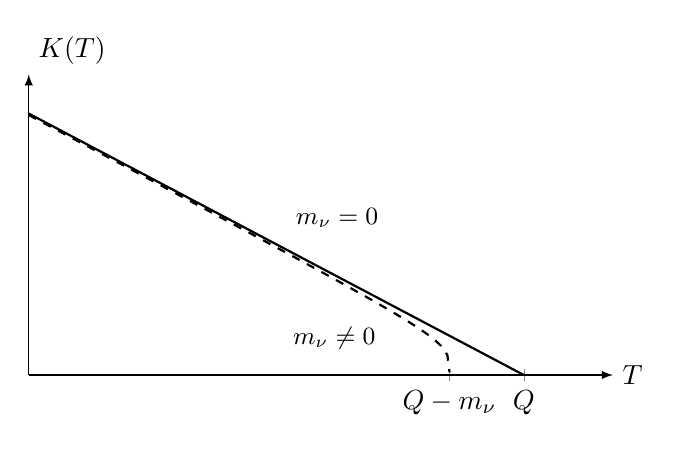
\begin{tikzpicture}
\begin{axis}[
    width=9cm, height=5.4cm,
    axis lines=left, axis line style={-latex},
    xlabel={$T$}, ylabel={$K(T)$},
    xlabel style={at={(ticklabel* cs:1)}, anchor=west},
    ylabel style={at={(ticklabel* cs:1)}, anchor=south west, rotate=-90},
    xmin=0, xmax=1.18, ymin=0, ymax=1.15,
    xtick={0.85,1}, xticklabels={$Q-m_\nu$,$Q$}, ytick=\empty,
    clip=false,
]
\addplot[black, thick, domain=0:1, samples=2] {1-x};
\addplot[black, thick, dashed, domain=0:0.85, samples=200]
    {sqrt((1-x)*sqrt(max((1-x)^2-0.0225,0)))};
\node[anchor=west, font=\small] at (axis cs:0.52,0.60) {$m_{\nu} = 0$};
\node[anchor=north east, font=\small] at (axis cs:0.72,0.22) {$m_{\nu} \neq 0$};
\end{axis}
\end{tikzpicture}
\caption{Diagramma di Kurie, con e senza massa del neutrino.}
\label{fig:kurie}
\end{figure}

Lo spettro misurato non coincide però esattamente con la \eqref{eq:spettro_beta}, perché il calcolo fatto trascura due effetti. 

Il primo è l'interazione coulombiana tra la particella $\beta$ e il nucleo figlio, che attrae gli elettroni e respinge i positroni: si osservano quindi più elettroni di bassa energia e meno positroni di bassa energia di quanti ne preveda il conto. Si tiene conto di questo effetto introducendo un fattore moltiplicativo, la funzione di Fermi $F(Z',p)$\mkeyword{funzione di Fermi}, dove $Z'$ è il numero atomico del nucleo figlio. 

Il secondo è la dipendenza dell'elemento di matrice dagli impulsi, che abbiamo trascurato con l'approssimazione permessa. In alcuni casi $M_{fi}$ si annulla in questa approssimazione e bisogna tenere i termini successivi dello sviluppo delle onde piane: si parla allora di decadimenti \emph{proibiti}\mkeyword{decadimento proibito}, che non sono realmente vietati ma solo meno probabili, e quindi caratterizzati da vite medie più lunghe. 

Lo spettro $\beta$ completo contiene quindi tre fattori
%
\begin{tcolorbox}[colback=yellow!10!white, colframe=orange!70!black, boxrule=0.8pt]
\begin{equation}
    N(p) \propto \underbrace{p^2 (Q - T)^2}_{\text{fattore statistico}} \cdot \underbrace{F(Z',p)}_{\text{campo coulombiano}} \cdot \underbrace{|M_{fi}|^2 S(p,q)}_{\text{elemento di matrice}}
\end{equation}
\end{tcolorbox}

